\documentclass[12pt, a4paper, twoside]{scrartcl}
 %---- Allgemeine Layout Einstellungen ------------------------------------------

% Für Kopf und Fußzeilen, siehe auch KOMA-Skript Doku
\usepackage[komastyle]{scrpage2}
\pagestyle{scrheadings}
\setheadsepline{0.5pt}[\color{black}]


%Einstellungen für Figuren- und Tabellenbeschriftungen
\setkomafont{captionlabel}{\sffamily\bfseries}
\setcapindent{0em}


%---- Weitere Pakete -----------------------------------------------------------
% Die Pakete sind alle in der TeX Live Distribution enthalten. Wichtige Adressen
% www.ctan.org, www.dante.de

% Sprachunterstützung
\usepackage[ngerman]{babel}

% Benutzung von Umlauten direkt im Text
% entweder "latin1" oder "utf8"
\usepackage[utf8]{inputenc}

% Pakete mit Mathesymbolen und zur Beseitigung von Schwächen der Mathe-Umgebung
\usepackage{latexsym,exscale,stmaryrd,amssymb,amsmath}

% Weitere Symbole
\usepackage[nointegrals]{wasysym}
\usepackage{eurosym}

% Anderes Literaturverzeichnisformat
%\usepackage[square,sort&compress]{natbib}

% Für Farbe
\usepackage{color}

% Zur Graphikausgabe
%Beipiel: \includegraphics[width=\textwidth]{grafik.png}
\usepackage{graphicx}

% Text umfließt Graphiken und Tabellen
% Beispiel:
% \begin{wrapfigure}[Zeilenanzahl]{"l" oder "r"}{breite}
%   \centering
%   \includegraphics[width=...]{grafik}
%   \caption{Beschriftung} 
%   \label{fig:grafik}
% \end{wrapfigure}
\usepackage{wrapfig}

% Mehrere Abbildungen nebeneinander
% Beispiel:
% \begin{figure}[htb]
%   \centering
%   \subfigure[Beschriftung 1\label{fig:label1}]
%   {\includegraphics[width=0.49\textwidth]{grafik1}}
%   \hfill
%   \subfigure[Beschriftung 2\label{fig:label2}]
%   {\includegraphics[width=0.49\textwidth]{grafik2}}
%   \caption{Beschriftung allgemein}
%   \label{fig:label-gesamt}
% \end{figure}
\usepackage{subfigure}

% Caption neben Abbildung
% Beispiel:
% \sidecaptionvpos{figure}{"c" oder "t" oder "b"}
% \begin{SCfigure}[rel. Breite (normalerweise = 1)][hbt]
%   \centering
%   \includegraphics[width=0.5\textwidth]{grafik.png}
%   \caption{Beschreibung}
%   \label{fig:}
% \end{SCfigure}
\usepackage{sidecap}
\usepackage{float}

% Befehl für "Entspricht"-Zeichen
\newcommand{\corresponds}{\ensuremath{\mathrel{\widehat{=}}}}
\newcommand{\folgt}{\ensuremath{\mathrel{\Rightarrow}}}
\newcommand{\equals}{\ensuremath{\mathrel{\Leftrightarrow}}}
\newcommand{\degree}{\ensuremath{\mathrel{^{\circ}}}}

\newcommand{\nn}{\nonumber}
\newcommand{\tn}[1]{\textnormal{#1}}
\newcommand{\D}{\ensuremath{\mathrel{\rm d}}}

\newcommand{\const}{\tn{const}}

\newcommand{\meter}{\ensuremath{\mathrel{\tn m}}}
\newcommand{\kilogramm}{\ensuremath{\mathrel{\tn{kg}}}}
\newcommand{\second}{\ensuremath{\mathrel{\tn s}}}
\newcommand{\sekunde}{\second}

\newcommand{\volt}{\ensuremath{\mathrel{\tn V}}}
\newcommand{\pascal}{\ensuremath{\mathrel{\tn{Pa}}}}
\newcommand{\coulomb}{\ensuremath{\mathrel{\tn C}}}
\newcommand{\newton}{\ensuremath{\mathrel{\tn N}}}
\newcommand{\liter}{\ensuremath{\mathrel{\tn l}}}
\newcommand{\celsius}{\ensuremath{\mathrel{\tn C}}}
\newcommand{\fahrenheit}{\ensuremath{\mathrel{\tn F}}}
\newcommand{\joule}{\ensuremath{\mathrel{\tn J}}}
\newcommand{\kelvin}{\ensuremath{\mathrel{\tn K}}}
\newcommand{\mol}{\ensuremath{\mathrel{\tn{mol}}}}
\newcommand{\gramm}{\ensuremath{\mathrel{\tn{g}}}}

\newcommand{\kilo}{\ensuremath{\mathrel{\tn k}}}
\newcommand{\hecto}{\ensuremath{\mathrel{\tn h}}}

\newcommand{\centi}{\ensuremath{\mathrel{ \tn c}}}
\newcommand{\milli}{\ensuremath{\mathrel{ \tn m}}}
\newcommand{\micro}{\ensuremath{\mathrel{ \tn\mu }}}



%\newcommand{}{\ensuremath{\mathrel{  }}}
%\newcommand{}{\ensuremath{\mathrel{  }}}
%\newcommand{}{\ensuremath{\mathrel{  }}}


\newcommand{\person}[1]{\textsc{#1}}

 \begin{document}
 %Titelseite
\begin{titlepage}
\centering
\textsc{\Large Anfängerpraktikum der Fakultät für
  Physik,\\[1.5ex] Universität Göttingen}

\vspace*{4.2cm}

\rule{\textwidth}{1pt}\\[0.5cm]
{\huge \bfseries
  Spezifische Wärme der Luft und Gasthermometer}\\[0.5cm]
\rule{\textwidth}{1pt}

\vspace*{3.5cm}

\begin{Large}
\begin{tabular}{ll}
Praktikanten: &  Silke Andrea Teepe\\
& Marcel Kramer\\
E-Mail: & \\
Betreuer: & Alexander Schmelev\\
\end{tabular}
\end{Large}

\vspace*{0.8cm}

\begin{Large}
\fbox{
  \begin{minipage}[t][2.5cm][t]{6cm} 
    Testat:
  \end{minipage}
}
\end{Large}

\end{titlepage}
\cleardoublepage
\tableofcontents
\cleardoublepage
\setcounter{page}{1}

\section{Einleitung}
\label{sec:einleitung}

\section{Theorie}
\label{sec:theorie}
\subsection{Trägheitsmomente}
Das Trägheitsmoment des Rades (s. Abb. \ref{g:1}) bezüglich der Symmetrieachse $I_{R_{||}}$ kann hergeleitet werden, indem man die Bewegung in Zylinderkoordinaten betrachtet:\\
\begin{align*}
 J_{R_{||}} &= \int \limits_{M_R} r^2_{\perp} \tn{d}x = \rho_R \int \limits_{V_R} r^2_{\perp} \tn{d} V \\
 &=\rho_R \int \limits_0^{D_R} \int \limits_0^{2\pi} \int \limits_0^{R_R} r^3 \tn{d}r \tn{ d}\varphi \tn{ d}z = \rho_R \int \limits_0^{D_R} \int \limits_0^{2\pi} \frac{1}{4} R^4_R \tn{ d}\varphi \tn{ d}z  \\
 &= \rho_R \int \limits_0^{D_R} \frac{1}{2}\pi R^4_R \tn{d}z = \rho_R D_R \frac{1}{2} \pi R^4_R \\
 &= \frac{1}{2} M_R R^2_R 
\end{align*}
Es entspricht dabei $M_R = \rho_R D_R \pi R^2_R$ der gesamten Masse des Rades, $\rho_R$ dessen Dichte, $R_R$ dem Radius und $D_R$ der Dicke.\\
\newline
Das vertikale Trägheitsmoment des gesamten Versuchsaufbaus $J_{ges_\perp}$ bezüglich der Aufhänung benötigt zur Bestimmung zunächst das Trägheitsmoment eines Zylinders um eine Achsensenkrechte der Symmetrieachse durch den Schwerpunkt \protect\footnotemark:\\
\begin{align*}
 J_{Z_{\perp}} &= M \left( \frac{1}{12} D^2 + \frac{1}{4} R^2 \right)
\end{align*}
Hier entspricht $D$ der Dicke, $R$ dem Radius und $M$ der Masse des Zylinders.\\
Mit Hilfe des Steiner'schen Satzes kann nun $J_{ges_\perp}$ bestimmt werden. Das Trägheitsmoment des Stabes wird dabei vernachlässigt.\\
\begin{align*}
 J_{ges_\perp} &= J_{R_{\perp}} + M_R \tn{ d}^2_R + J_{A_{\perp}} + M_A \tn{ d}^2_A  \\
 &= M_R \left( \frac{1}{12} D^2_R + \frac{1}{4} R^2_R + \tn{ d}^2_R \right) + M_A \left( \frac{1}{12} D^2_A + \frac{1}{4} R^2_A + \tn{ d}^2_A \right)
\end{align*}
($d_R \hat{=}$ Abstand Unterstützungspunkt zum Radschwerpunkt; $J_{A_{\perp}} \hat{=}$ vertikales Trägheitsmoment des Ausgleichgewichts; $D_A \hat{=}$ Dicke des Ausgleichgewichts; $R_A \hat{=}$ Radius des Ausgleichgewichts; $d_A \hat{=}$ Abstand Unterstützungspunkt zum Schwerpunkt des Ausgleichgewichts)\\
Aus Versuch 3 ist die Formel zur Berechnung des Trägheitsmoments $J_{R_{||}}$ eines physikalischen Radpendels bezüglich seiner Symmetrieachse bekannt:\\
\begin{align}
\label{eq:phypendel}
 J_{R_{||}} &= \frac{g d_P m_P T^2}{4 \pi^2} - m_P d^2_P
\end{align}
($T \hat{=}$ Schwingungsdauer des Rades; $d_P \hat{=}$ Abstand Pendelgewicht zur Drehachse; $m_P \hat{=}$ Masse des Pendelgewichts)\\

\subsection{Präzession}
Durch das angehängte Zusatzgewicht wird auf den Versuchsaufbau ein Drehmoment\\
\begin{align*}
 |\overrightarrow{D} = | d_Z \tn{x} \overrightarrow{F_G} = d_Z  m_Z  g \tn{sin}\left( \Theta \right)
\end{align*}
($d_Z \hat{=}$ Abstand Zusatzgewicht zur vertikalen Drehachse; $F_G \hat{=}$ Gewichtskraft auf das Zusatzgewicht; $m_Z \hat{=}$ Masse des Zusatzgewichts; $\Theta \hat{=}$ Winkel zwischen Stab und vertikaler Drehachse) ausgeübt. $\overrightarrow{D}$ steht senkrecht auf dem Drehimpuls $\overrightarrow{L}$ des Rades und ändert, da $\frac{\tn{d}\overrightarrow{L}}{\tn{d} t} = \overrightarrow{D}$, nicht den Betrag, sondern lediglich die Richtung. Somit überstreicht die Drehimpulsachse einen Kegel; normiert man die Seitenlänge diesens auf $L$, so ergibt sich für den Radius des nach oben breiter werdenden Kegels $L \cdot \tn{sin} \left( \Theta \right)$. Betrachten des Winkels $\alpha$ (im Bogenmaß), der innerhalb eines bestimmten Zeitintervalls  von der Drehachse eingeschlossen wird, ergibt folgenden Zusammenhang:\\
\begin{align*}
\omega_P &= \frac{\tn{d} \alpha}{\tn{d} t} = \frac{\frac{\tn{d} L}{\tn{d} t}}{L \tn{sin} \left( \Theta \right)} = \frac{D}{L \tn{sin} \left( \Theta \right)} \\
&= \frac{d_Z m_Z g \cdot \tn{sin} \left( \Theta \right)}{ J_{R_{||}} \omega_R \cdot \tn{sin} \left( \Theta \right)}\\
&= \frac{d_Z m_Z g}{J_{R_{||}} \omega_R}
\end{align*}
($\omega_P \hat{=}$ Winkelgeschwindigkeit der Präzession; $\omega_R \hat{=}$ Winkelgeschwindigkeit des Rades bezüglich der Symmetrieachse) Es folgt für das waaerechte Trägheitsmoment des Rades bezüglich seiner Symmetrieachse:\\
\begin{align}
\label{eq:kreisel}
 J_{R_{||}} &= \frac{d_Z m_Z g}{\omega_P \omega_R}
\end{align}

\subsection{Nutation}
Die Figurenachsen bezeichnen die Achsen bezüglich denen ein Körper das kleinste oder größte Trägheitsmoment besitzt. Lediglich Rotation um diese Achsen ist stabil. Verschieben der Drehimpulsachse aus einer parallelen Lage zu einer Figurenachse, z.B. durch einen Stoß, führt zu einer Rotation der Figurenachse um die Drehimpulsachse. Sichtbar wird dies durch ``Wippen'', bzw. ``Nicken'' des Kreisels.  \\
Sei $\overrightarrow{\omega_N}$ die Winkelgeschwindigkeit der Nutation, $\overrightarrow{\omega_{N_{\perp}}}$ den vertikaln Anteil dieser, und $\alpha$ der Winkel zischen $\overrightarrow{\omega_N}$ und $\overrightarrow{\omega_R}$. $\overrightarrow{L_{||}}$ sei der horizontale Anteil von $\overrightarrow{L}$, parallel zu $\overrightarrow{\omega_R}$; $\overrightarrow{L_{\perp}}$ sei der vertikale Anteil, parallel zu $\overrightarrow{\omega_{N_{\perp}}}$. $\overrightarrow{J_{{Ges}_{||}}}$ und $\overrightarrow{J_{{Ges}_{\perp}}}$ seien nach dem gleichen Prizip definiert. Es gelten die folgenden Zusammenhänge:\\
\begin{align*}
 \overrightarrow{\omega_{N_{\perp}}} &= \overrightarrow{\omega_N} \cdot \tn{sin} \left( \alpha \right) \\
 \frac{L_{||}}{\tn{cos} \left( \alpha \right)} &= L = \frac{L_{\perp}}{\tn{sin} \left( \alpha \right)} \\
 L_{||} &= J_{{Ges}_{||}} \cdot \omega_R \\
 L_{\perp} &= J_{{Ges}_{\perp}} \cdot \omega_{N_{\perp}} \\
 \equals \omega_N &= \frac{\omega_{N_{\perp}}}{\tn{sin} \left( \alpha \right)} = \frac{L_{\perp}}{J_{{Ges}_{\perp}}\tn{sin} \left( \alpha \right)} = \frac{L_{||}}{J_{{Ges}_{\perp}} \tn{cos} \left( \alpha \right)}\\
 &= \frac{J_{{Ges}_{||}} \omega_R}{J_{{Ges}_{\perp}} \tn{cos} \left( \alpha \right)}
\end{align*}
Für kleine Auslenkwinkel $\alpha$ ist $\tn{cos} \left( \alpha \right) \approx 1$. Damit folgt:\\
\begin{align}
\label{eq:nutation}
 \frac{\omega_N}{\omega_R} &\approx \frac{J_{{Ges}_{||}}}{J_{{Ges}_{\perp}}}
\end{align}





\section{Durchführung}
\label{sec:durchfuehrung}



\section{Auswertung}
\label{sec:auswertung}
\subsection{Theoretische Berechnung des Trägheitsmomentes}

Wie aus dem Versuch "Das Trägheitsmoment" bekannt ist berechnet sich das horizontale Trägheitsmoment eines Rades mit Masse $M_R$ und Radius $R_R$ durch die Formel
\begin{align*}
J_{hor}=\frac{1}{2}M_RR_R^2.
\end{align*}
Mit den abgelesenen Werten des Rades aus Tabelle \ref{tab:datenrad} erhält man $J=9,95\cdot10^{-3}$. Die abgelesenen Werte waren ohne Fehlerangaben und werden daher als exakt angenommen. Der Messfehler für die selbst gemessenen Längen wurde mit $2\milli\meter$ abgeschätzt.

\renewcommand{\arraystretch}{1.2}
\begin{table}[H]
\centering
\begin{tabular}{|l|c||}
	\hline
    Größe & Wert  \\
    \hline\hline
    Masse des Rads $M_R$ & $1326\gramm$  \\
    \hline
    Masse des Zusatzgewichts $M_Z$ & $80\gramm $  \\
    \hline
    Masse des Ausgleichsgewichts $M_G$ & $932\gramm$  \\
    \hline
    Breite des Rads $L_R$ & $28\milli\meter$  \\
    \hline
    Abstand Rad zum Stützpunkt $A_R$ & $11,5\centi\meter $  \\
    \hline
    Abstand Ausgleichsgewicht zum Stützpunkt $A_G$ & $16,8\pm0,2\centi\meter $  \\
    \hline
    Länge des Ausgleichsgewichts $L_G$ & $4,35\pm0,2\centi\meter $  \\
    \hline
    Länge des Stabs $L_S$ & $40\pm0,2\centi\meter $  \\
    \hline	
    Radius des Rads $R_R$ & $245\milli\meter$  \\
    \hline
    Radius des Ausgleichsgewichts $R_G$ & $3\pm0,2\centi\meter$  \\
    \hline
 \end{tabular} 
 \caption{\label{tab:datenrad}Werte  zur Berechnung der Trägheitsmomente}
\end{table}

Um das vertikale Trägheitsmoment des Kreisels zu bestimmen wird die Summe aus den Trägheitsmomenten der Komponenten gebildet und der Satz von Steiner ausgenutzt. Dabei werden Rad und Ausgleichsgewicht als Zylinder betrachtet, deren Trägheitsmoment bei Rotation durch die Mittelachse $J_Z=\frac{1}{4}MR^2+\frac{1}{12}ML^2$ beträgt. Das Trägheitsmoment eines Stabes ist $J_S=\frac{1}{12}ML^2$. Insgesamt erhält man
\begin{align*}
J_{vert}&=J_{Rad}+J_{Ausgleichgewicht}+J_{Stange}\\
			&=\frac{1}{4}M_RR_R^2+\frac{1}{12}M_RL_R+M_RA_R+\frac{1}{4}M_GR_G^2+\frac{1}{12}M_GL_G^2+M_GA_G\\
			&\hspace{0.4cm}+\frac{1}{12}M_SL_S^2+M_S\left(\frac{L_S}{2}-L_R\right)^2.
\end{align*}
%Der Fehler wird durch Fehlerfortpflanzung ermittelt
%Fehler wirklich hinschreiben? Falls nicht den Satz hierdrüber vor dem Ergebnis schieben.
%\begin{align*}
%\sigma_{J_{vert}}^2=\left(2M_RA_R-2M_S\left(\frac{L_S}{2}-L_R\right)\right)^2\sigma_{L_R}^2+
%\end{align*}
Die Masse der Stange lies sich leider nicht genau bestimmen und muss daher abgeschätzt werden. Ihr Volumen ist $(V=\pi R^2\cdot L)$. Die Stange ist vermutlich aus Eisen, was eine Dichte von $7,874\frac{g}{\centi\meter^2}$ besitzt, wie man in jedem Nachschlagewerk sehen kann. Einsetzten unserer Werte liefert $M_S=247,37\gramm$. Wir schätzen den Wert daher mit $M_S=\left(250\pm100\right)\gramm$ ab. Der Gesamtfehler $\sigma_{J_{vert}}$ des Trägheitsmomentes ergibt sich aus der Fehlerfortpflanzung. Das Ergebnis mit den gemessenen Werten ist
\begin{align*}
J_{vert}=\left(6,93\pm0,12\right)\cdot10^{-3}\kilo\gramm\,\meter^2.
\end{align*}

\subsection{Berechnung des Trägheitsmomentes als physikalisches Pendel}
%Aus Formel \ref{eq:phypendel} erhält man für das Trägheitsmoment des physikalischen Pendels
%%%%%%%%%%%%Alte Formel aus Theorie dazu %%%%%%%%%%%
%\begin{align}
%\label{eq:phypendel}
%T=2\pi\sqrt{\frac{J}{Mgd}}
%\end{align}
%%%%%%%%%%%%%%%%%%%%%%%%%%%%%%%%%%%%%%%%%%%%%%%%%%%%
%\begin{align*}
%J=\frac{MgdT^2}{4\pi^2}.
%\end{align*}
%Dabei ist T die Periodendauer, d der Abstand zur Drehachse und g die Erdbeschleunigung. Bei dem für den Versuch verwendeten Aufbau muss noch die Masse des Zusatzgewichtes beachtet werden und der Satz von Steiner angewandt werden, um den Abstand $a$ des Zusatzgewichtes zur Drehachse zu beachten. Die Formel lautet also
%\begin{align*}
%J=\frac{\left(M_R+M_G\right)gd}{4\pi^2}-M_Ga^2.
%\end{align*}
%--------------------------------------------------------------

Das Trägheitsmoment des physikalischen Pendels lässt sich mit Formel \ref{eq:phypendel} berechnen. Bei dem verwendeten Versuchsaufbau lautet sie
\begin{align*}
J=\frac{\left(M_R+M_G\right)gdT^2}{4\pi^2}-M_GA_G^2.
\end{align*}
Dabei ist T die Periodendauer, d der Abstand zur Drehachse und g die Erdbeschleunigung. Der Abstand zur Drehachse $d$ berechnet sich zu
\begin{align*}
d=\frac{M_G}{M_R+M_G}\cdot A_G=\left(0,0096\pm0,0001\right)\meter.
\end{align*}
Die Periodendauer $T=1,69\pm0,014\second$ ergibt sich aus den gewichteten Mittelwert der Messungen. Der zugehörige systematische Fehler wurde durch $\sigma_T=0,01+0,005t$ abgeschätzt. Für das Trägheitsmoment ergibt sich damit
\begin{align*}
J=\left(9,16\pm1,99\right)\cdot10^{-3}\kilo\gramm\,\meter^2.
\end{align*}



%\subsection{Berechnung des Trägheitsmomentes durch die Kreiselpräzission}
\subsection{Präzessionsfrequenz}
Im zweiten teil wurde die je eine halbe Periodendauer $T_p$ der Präzession und die Periodendauer $T_r$ der Rotation des Rades nach jeweils einer halben Umdrehung des Kreisels gemessen. Aus diesen Messungen ergeben sich die Präzessionsfrequenz $\omega_p=\frac{2\pi}{T_p}$ und die Rotationsfrequenz $\omega_r=\frac{2\pi}{T_r}\Leftrightarrow\omega_r^{-1}=\frac{T_r}{2\pi}$. Um die Rotationsfrequenz während der Präzessionsmessung zu erhalten wird zu jedem Messwert der Präzession jeweils der Mittelwert aus der Rotationsfrequenz vorher und hinterher gebildet. Der Fehler $\sigma_{T_r}$ der Rotation ergibt sich durch Fehlerfortpflanzung zu $\sigma_{\omega_r}=\frac{2\pi}{T_r^2}\sigma_{T_r}$. Analog berechnet sich der Fehler der Präzession zu$\sigma_{T-p}=\frac{2\pi}{T_p^2}\sigma_{T_p}$. Für den Fehler $\sigma_T$ der Zeitmessung mit der Lichtschranke wurde wie oben wieder der systematische Fehler $\sigma_T=0,01+0,005t$ verwendet. Die Ergebnisse sind in Abbildung \ref{fig:kreisel} zu sehen. Die steigung der zugehörigen Regressionsgeraden ergibt sich jeweils durch $\Omega=\omega_r\omega_p$.
\begin{figure} [H]
\centering
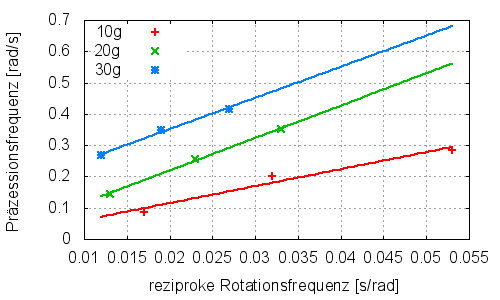
\includegraphics[scale=0.8]{kreisel.png}
\caption{\label{fig:kreisel}Verhältnis von Rotations- und Präzessionsfrequenz}
\end{figure}


Nun lässt sich das Trägheitsmoment mithilfe von Formel \ref{eq:kreisel} aus dem Theorieteil berechnen. Der Abstand vom Zusatzgewicht zur Drehachse beträgt $d_Z=\left(28,5\pm0,2\right)cm$. Der Fehler des Trägheitsmoment ist
\begin{align*}
\sigma_J=\sqrt{\left(\frac{m_Zg}{\omega_r\omega_p}\right)^2\sigma_r^2+\left(\frac{d_Zm_Zg}{(\omega_p\omega_r)^2}\right)^2\sigma_\Omega^2}
\end{align*}
Die Trägheitsmomente der einzelnen Massen sind in Tabelle \ref{tab:kreisel} aufgeführt. Berechnet man den gewichteten Mittelwert erhält man
\begin{align*}
J=\left(9,77\pm0,40\right)\cdot10^{-3}\kilo\gramm\,\meter^{-2}.
\end{align*}



\renewcommand{\arraystretch}{1.0}
\begin{table}[H]
\centering
\begin{tabular}{|c|c|}
	\hline
    Masse [g] & Trägheitsmoment J [$\kilo\gramm\,\meter^{-2}\cdot10^{-3}$]  \\
    \hline\hline
     10 & $10,07\pm0,71$  \\
     20 & $10,37\pm0,72$  \\
     30 & $0,91\pm0,64$  \\
    \hline
 \end{tabular} 
 \caption{\label{tab:kreisel}Trägheitsmomente aus Messung 4 und 5}
\end{table}

\subsection{Nutation}
Die Nutationsgeschwindigkeit lässt sich durch
\begin{align*}
\omega_n=\frac{2\pi}{T_n}
\end{align*}
mit dem Fehler $\sigma_{\omega_n}=\sigma_{T_n}\frac{2\pi}{T_n^2}$ berechnen. Dabei wird wieder der systematische Fehler der Stoppuhr mit $\sigma_{T_n}=0,01+0,005t$ beachtet. In Abbildung \ref{fig:nutation} sind die Ergebnisse zu sehen. Man kann einen linearen Zusammenhang erkennen, auch wenn der zweit Messwert etwas abzuweichen scheint.

\begin{figure} [H]
\centering
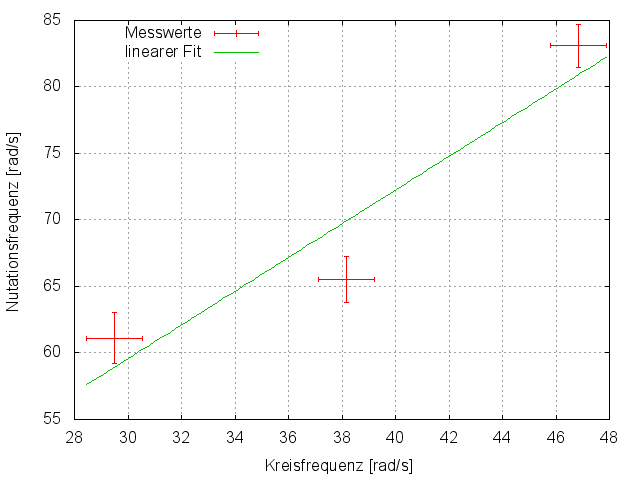
\includegraphics[scale=0.8]{nutation.png}
\caption{\label{fig:nutation}Rotations- und Nutationsfrequenz}
\end{figure}

Die lineare Regression ergibt den Wert $m=1,27$ für die Regressionsgerade. Nach Gleichung \ref{eq:nutation} gilt die Näherung
\begin{align*}
m= \frac{\omega_N}{\omega_R} &\approx \frac{J_{{Ges}_{||}}}{J_{{Ges}_{\perp}}}
\end{align*}
womit sich unter verwendung des vorher bestimmten horizontalen Trägheitsmoment $J_{{Ges}_{||}}$ nun das vertikale Trägheitsmoment $J_{{Ges}_{\perp}}$ bestimmen lässt. Man kommt auf
\begin{align*}
J_{{Ges}_{\perp}}=\left(7,2\pm0,5\right)\cdot10^{-3}\kilo\gramm\,\meter^{-2}.
\end{align*}






\section{Diskussion}
\label{sec:diskussion}
In Tabelle \ref{tab:ergebnisse} sind die drei berechneten Werte für das horizontale Trägheitsmoment aufgeführt.

\renewcommand{\arraystretch}{1.0}
\begin{table}[H]
\centering
\begin{tabular}{|c|c|}
	\hline
    Messmethode & Trägheitsmoment J [$\kilo\gramm\,\meter^{-2}\cdot10^{-3}$]  \\
    \hline\hline
     theoretische Berechnung & $9,95$  \\ \hline
     physikalisches Pendel & $9,16\pm1,99$  \\ \hline
     Präzessionsmessung & $9,77\pm0,40$  \\ \hline
    \hline
 \end{tabular} 
 \caption{\label{tab:ergebnisse}Ergebnisse für das horizontale Trägheitsmoment}
\end{table}

Der theoretische Wert liegt im Fehlerintervall beider durch die Messwerte bestimmten Trägheitsmomente, daher ist anzunehmen das die Ergebnisse dem wahren Trägheitsmoment sehr nahe kommen.\\

Das Ergebnis der Nutationsmessung von $J_{n}=\left(7,2\pm0,5\right)\cdot10^{-3}\kilo\gramm\,\meter^{-2}$ weicht um etwa 4\% von dem theoretisch berechneten Wert $J_{t}=\left(6,93\pm0,12\right)\cdot10^{-3}\kilo\gramm\,\meter^2$ ab und beide Fehlerintervalle überschneiden sich. 




%\section*{Literatur}

%[Dem I] Demtröder Wolfgang, Experimentalphysik 1, 6. Auflage

%\newpage
%\section*{Anhang}




\end{document}
